% ------------
% header
\documentclass{scrreprt}
% ------------
% packages
\usepackage{tikz-network}
\usepackage{tikz}
\usetikzlibrary{positioning}

\begin{document}





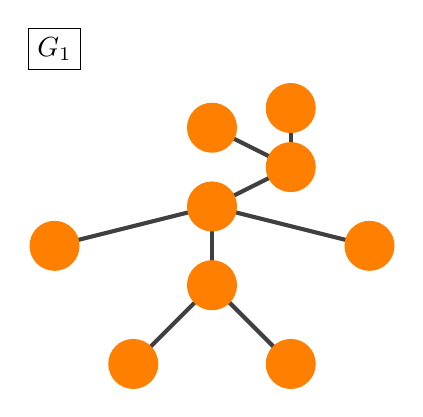
\begin{tikzpicture}
\node[draw] at (-1,4) {$G_1$};

	\Vertex[x=0,y=0,style={color = orange}]{A}
	\Vertex[x=2,y=0,style={color = orange}]{B}
     	\Vertex[x=1,y=1,style={color = orange}]{C} 
  	\Vertex[x=1,y=2,style={color=orange}]{D}
  	\Vertex[x=-1,y=1.5,style={color=orange}]{E}
   	\Vertex[x=3,y=1.5,style={color=orange}]{F}
  	\Vertex[x=2,y=2.5,style={color=orange}]{G}
     	\Vertex[x=2,y=3.25,style={color=orange}]{H}
      	\Vertex[x=1,y=3,style={color=orange}]{I}
	
      	\Edge(A)(C)
       	\Edge(B)(C)
        	\Edge(C)(D)
      	\Edge(E)(D)
     	\Edge(F)(D)
      	\Edge(G)(D)
       	\Edge(G)(H)
     	\Edge(G)(I)
\end{tikzpicture} \hspace{0.5cm} 
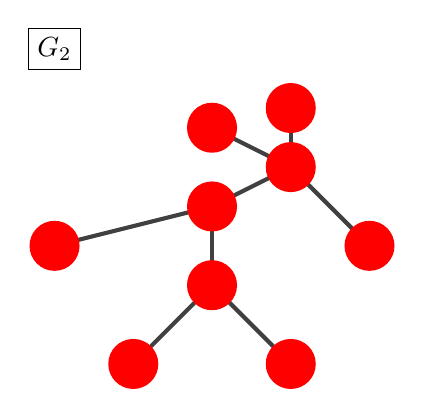
\begin{tikzpicture}
\node[draw] at (-1,4) {$G_2$};
	\Vertex[x=0,y=0,style={color = red}]{A}
	\Vertex[x=2,y=0,style={color = red}]{B}
     	\Vertex[x=1,y=1,style={color = red}]{C} 
  	\Vertex[x=1,y=2,style={color=red}]{D}
  	\Vertex[x=-1,y=1.5,style={color=red}]{E}
   	%\Vertex[x=3,y=1.5,style={color=red}]{F}
  	\Vertex[x=2,y=2.5,style={color=red}]{G}
     	\Vertex[x=2,y=3.25,style={color=red}]{H}
      	\Vertex[x=1,y=3,style={color=red}]{I}
	\Vertex[x=3,y=1.5,style={color=red}]{J}
	
      	\Edge(A)(C)
       	\Edge(B)(C)
        	\Edge(C)(D)
      	\Edge(E)(D)
     	%\Edge(F)(D)
      	\Edge(G)(D)
       	\Edge(G)(H)
     	\Edge(G)(I)
	\Edge(G)(J)
\end{tikzpicture} \hspace{0.5cm} 
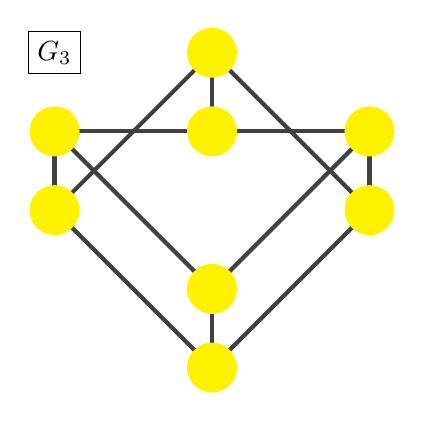
\begin{tikzpicture}
\node[draw] at (-2,4) {$G_3$};
	\Vertex[x=0,y=0,style={color = yellow}]{A}
	\Vertex[x=2,y=2,style={color = yellow}]{B}
	\Vertex[x=0,y=4,style={color = yellow}]{C} 
	\Vertex[x=-2,y=2,style={color=yellow}]{D}
	\Vertex[x=0,y=1,style={color=yellow}]{E}
	\Vertex[x=2,y=3,style={color=yellow}]{F}
	\Vertex[x=0,y=3,style={color=yellow}]{G}
	\Vertex[x=-2,y=3,style={color=yellow}]{H}
	
	\Edge(A)(B)
	\Edge(B)(C)
	\Edge(C)(D)
	\Edge(D)(A)
	\Edge(A)(E)
	\Edge(B)(F)
	\Edge(C)(G)
	\Edge(D)(H)
     	\Edge(E)(F)
	\Edge(F)(G)
	\Edge(G)(H)	
	\Edge(H)(E)
\end{tikzpicture}

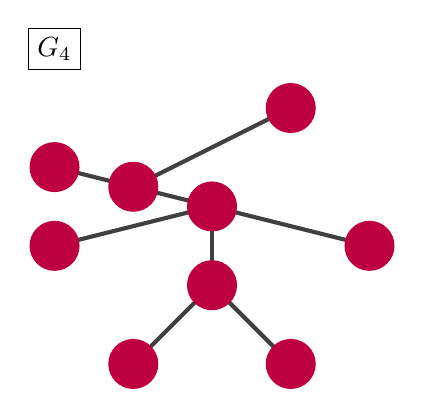
\begin{tikzpicture}
\node[draw] at (-1,4) {$G_4$};
	\Vertex[x=0,y=0,style={color = purple}]{A}
	\Vertex[x=2,y=0,style={color = purple}]{B}
     	\Vertex[x=1,y=1,style={color = purple}]{C} 
  	\Vertex[x=1,y=2,style={color=purple}]{D}
  	\Vertex[x=-1,y=1.5,style={color=purple}]{E}
   	\Vertex[x=3,y=1.5,style={color=purple}]{F}
  	\Vertex[x=0,y=2.25,style={color=purple}]{G}
     	\Vertex[x=2,y=3.25,style={color=purple}]{H}
      	\Vertex[x=-1,y=2.5,style={color=purple}]{I}
	
      	\Edge(A)(C)
       	\Edge(B)(C)
        	\Edge(C)(D)
      	\Edge(E)(D)
     	\Edge(F)(D)
      	\Edge(G)(D)
       	\Edge(G)(H)
     	\Edge(G)(I)
\end{tikzpicture} \hspace{0.5cm} 
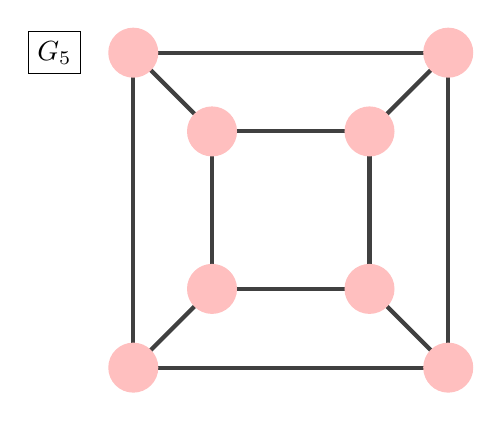
\begin{tikzpicture}
\node[draw] at (-1,4) {$G_5$};
	\Vertex[x=0,y=0,style={color = pink}]{A}
	\Vertex[x=4,y=0,style={color = pink}]{B}
	\Vertex[x=4,y=4,style={color = pink}]{C} 
	\Vertex[x=0,y=4,style={color=pink}]{D}
	\Vertex[x=1,y=1,style={color=pink}]{E}
	\Vertex[x=3,y=1,style={color=pink}]{F}
	\Vertex[x=3,y=3,style={color=pink}]{G}
	\Vertex[x=1,y=3,style={color=pink}]{H}
	
	\Edge(A)(B)
	\Edge(B)(C)
	\Edge(C)(D)
	\Edge(D)(A)
	\Edge(A)(E)
	\Edge(B)(F)
	\Edge(C)(G)
	\Edge(D)(H)
     	\Edge(E)(F)
	\Edge(F)(G)
	\Edge(G)(H)	
	\Edge(H)(E)
\end{tikzpicture} \hspace{0.5cm} 
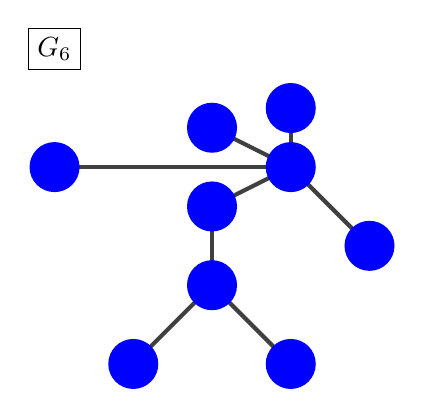
\begin{tikzpicture}
\node[draw] at (-1,4) {$G_6$};
	\Vertex[x=0,y=0,style={color = blue}]{A}
	\Vertex[x=2,y=0,style={color = blue}]{B}
     	\Vertex[x=1,y=1,style={color = blue}]{C} 
  	\Vertex[x=1,y=2,style={color=blue}]{D}
  	%\Vertex[x=-1,y=1.5,style={color=blue}]{E}
   	%\Vertex[x=3,y=1.5,style={color=blue}]{F}
  	\Vertex[x=2,y=2.5,style={color=blue}]{G}
     	\Vertex[x=2,y=3.25,style={color=blue}]{H}
      	\Vertex[x=1,y=3,style={color=blue}]{I}
	\Vertex[x=3,y=1.5,style={color=blue}]{J}
	\Vertex[x=-1,y=2.5,style={color=blue}]{K}
	
      	\Edge(A)(C)
       	\Edge(B)(C)
        	\Edge(C)(D)
      %	\Edge(E)(D)
     	%\Edge(F)(D)
      	\Edge(G)(D)
       	\Edge(G)(H)
     	\Edge(G)(I)
	\Edge(G)(J)
	\Edge(G)(K)
\end{tikzpicture}

%  \begin{scope}[red] 
%    \draw (0mm,0mm) -- (10mm,0mm); 
%    \draw (0mm,1mm) -- (10mm,1mm); 
%  \end{scope} 



  	



\end{document}